\subsection{Supernova Figure of Merit}
We compute the Dark Energy Task force figure of merit in the dark energy parameters $w_0-w_a.$
The supernova sample is simulated following roughly the same prescription as that outlined in the recent Science Requirements Document, with a few differences:
\begin{itemize}
\item host redshift selection function: for the SRD we adjusted the survey size simulated to ensure roughly 112 000 SNe after host selection cuts from a 4MOST-like ground based telescope. This is the largest determinant of the final size, and so in order to test for differences in the survey strategy we increased the survey size simulated (so that the host-$z$ follow up was not the most important characteristic).
\item colour cuts: in concert with the above, we impose a most restrictive cut on the fitted colour in the SAL2T fit from $\sigma(c) < 0.08$ to $\sigma(c) < 0.05.$ Insodoing we are forcing that the supernovae that survive are of higher quality than in the SRD.
\item including only statistical errors: for speed of computation we have neglected the astrophysical systematics; this will be relaxed in future versions
\end{itemize}

\begin{figure}
  \begin{center}
$\begin{array}{cc} 
    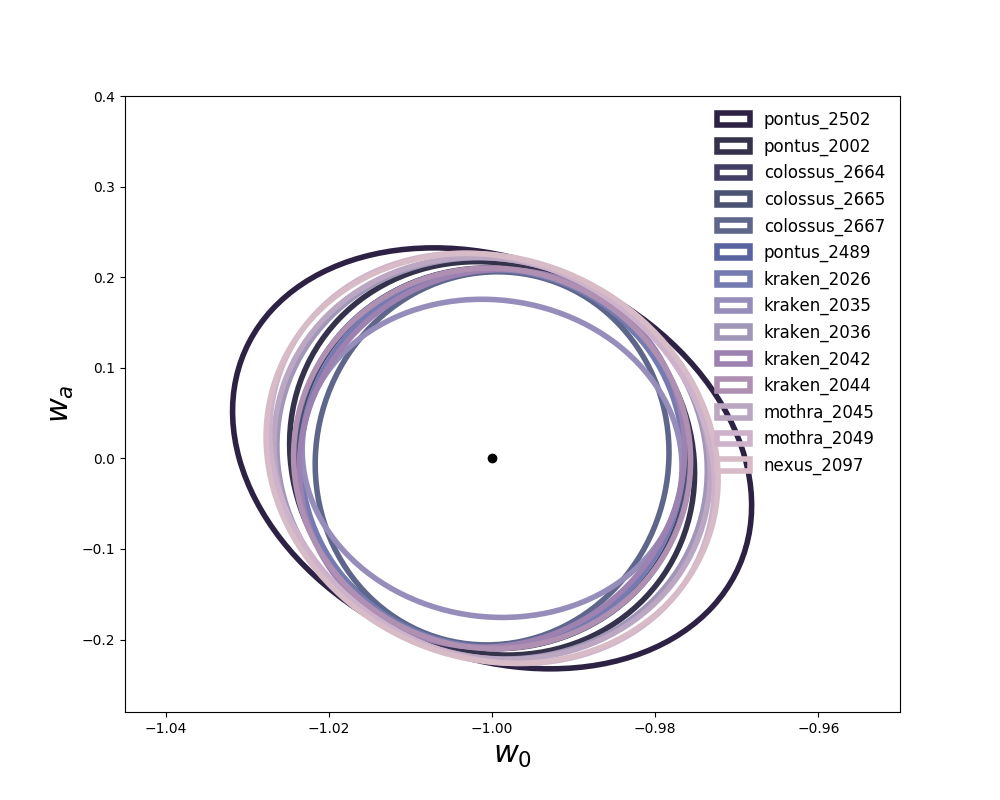
\includegraphics[width=0.45\textwidth]{Figures/FM_plot_cadence_updated.png} &
    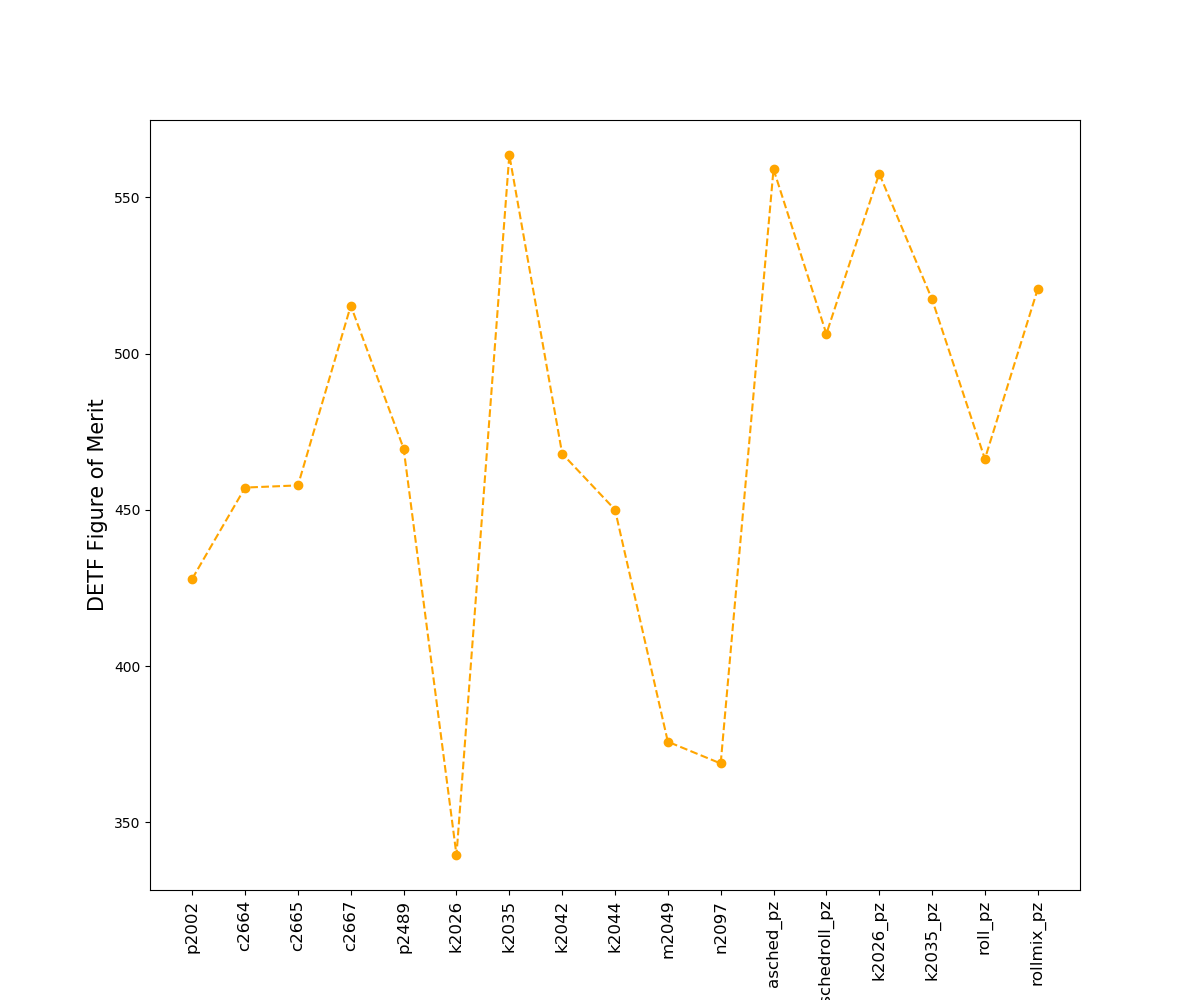
\includegraphics[width=0.4\textwidth]{Figures/FoM_cadence_updated.png}
\end{array}$
    \caption{Cosmology constraints across cadence types: the ellipses in the $w_0-w_a$ plane (left panel) and the dark energy figure of merit is shown (right panel) are shown. 
    \label{fig:snfom}}
  \end{center}
\end{figure}

The largest difference in the Figure of Merit we find is a factor of two between the highest FoM (kraken 2035) \textbf{[RH waiting for the runs to complete - don't think this is right for kraken as it is the least converged right now]} and the lowest FoM (pontus 2502). The lowest-performing strategy has two alternating bands in declination, switching in alternate years, which is expect to perform poorly. The highest performing strategy...  



